% Appendix A

\chapter{Extra material} % Main appendix title

\label{AppendixA} % For referencing this appendix elsewhere, use \ref{AppendixA}

%-----------------------------------
%	SECTION 1
%-----------------------------------
\section{Phase Problem} \label{sec:No_direcionality}
This section shows that a problem with the correspondence of a phase to an evolution exists.
It arises when Bottarelli's approach is directly implemented on an atomic system in \autoref{sec:challenges}.

\noindent
For $ N = 6 $ one can recreate the topology as in \autoref{fig:botarellis_topo}.
The phase $ \theta $ depends on the positions and dipole orientations of the three loop-atoms.
This dependence is shown in \autoref{fig:Theta_vs_d_phi_different_Evo} a).
Multiple combinations that lead to the same $ \theta $ have different evolutions,
which is depicted in \autoref{fig:Theta_vs_d_phi_different_Evo} b).
\begin{figure}[ht]
    \centering
    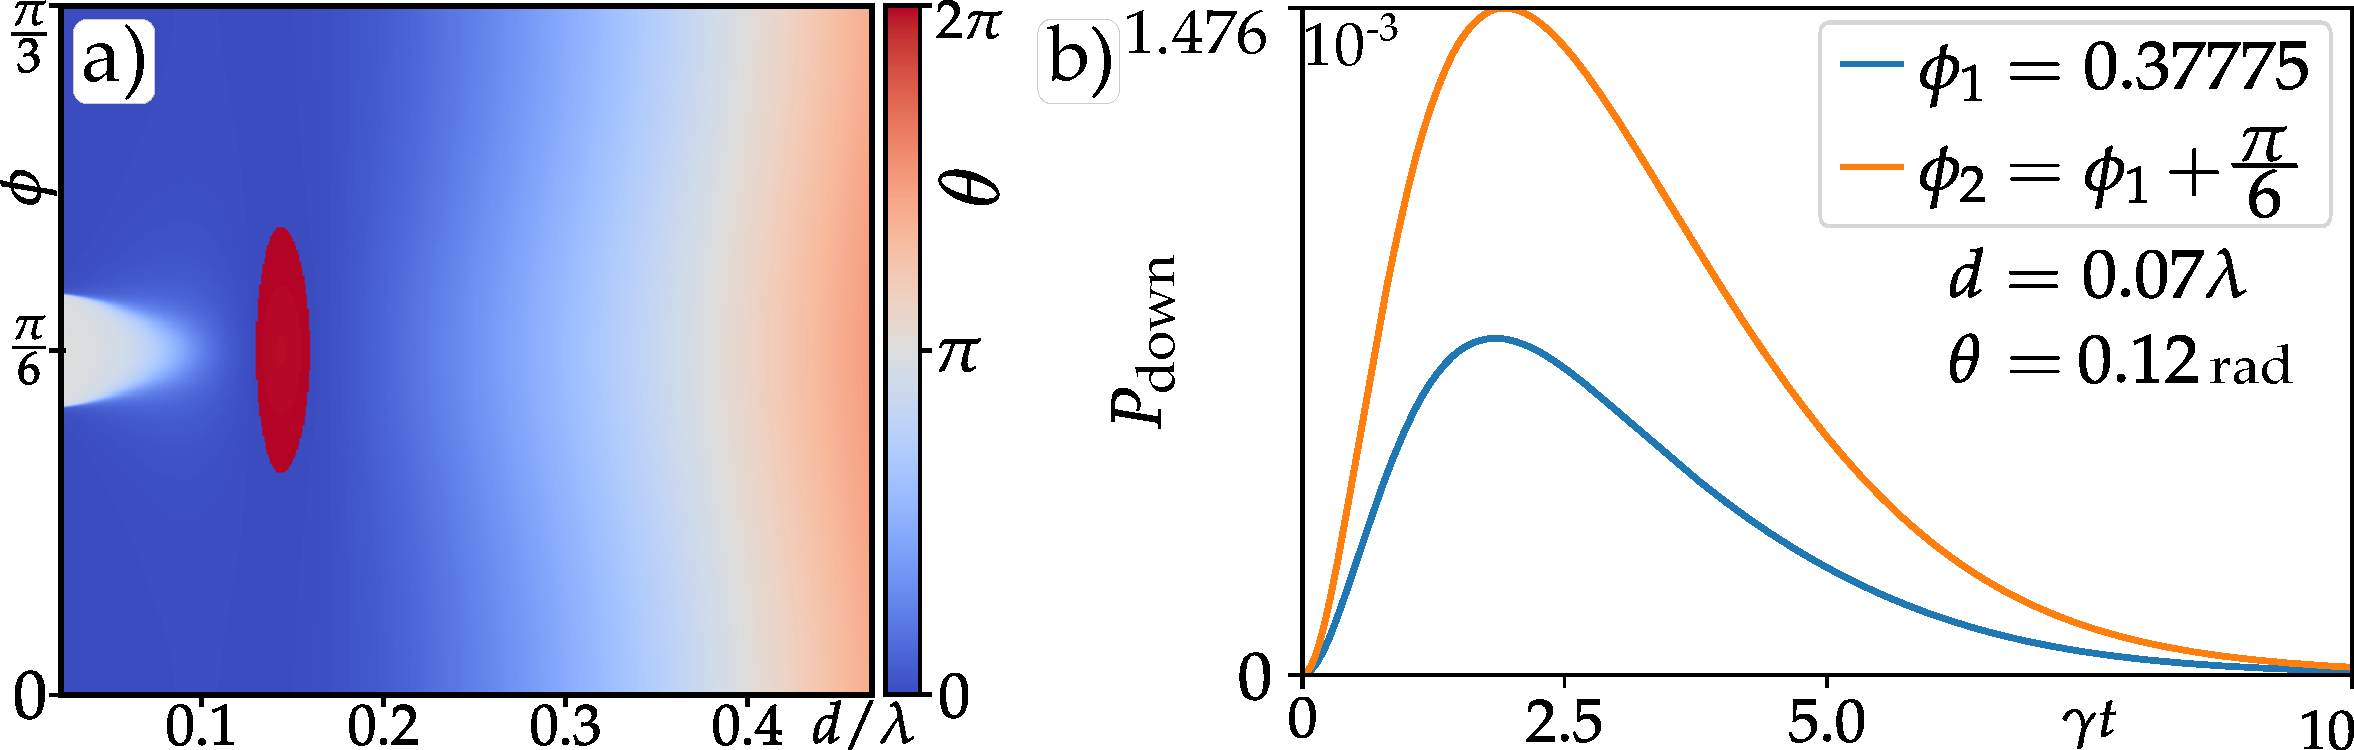
\includegraphics[width=\textwidth]{THETA(d,angle)_for_all_inner}
    \caption{The first plot (a) Shows the dependence of the phase in the loop for an equilateral triangle.
    The angle $ \phi $ measures the orientation of the dipoles with respect to the x-axis.
    Care must be taken, as multiple combinations of $d/\lambda$ and $ \phi $ can lead to the same $ \theta $ but result in different evolutions, as seen in (b).
    The second plot (b) shows the evolution of a classical state which is initially on the left arm, exactly like in \cite{Startingpoint}.}
    \label{fig:Theta_vs_d_phi_different_Evo}
\end{figure}
But again, changing the phase does not allow for directional routing in the first place.
The Hamiltonian for the atomic system is not hermitian and chirality is not possible.

\newpage
%-----------------------------------
%	SECTION 2
%-----------------------------------
\section{Diagonalization} \label{sec:Diagonalization}
The Hamiltonian of a infinite system can be diagonalized with a Fourier transformation.
This section shows that it is still useful to operate in $k$-space even for a finite system, as mentioned in section \ref{sec:Sys_def_N_bigger_6}.

\noindent
The matrices $ V $ and $ \Gamma $ described in section \ref{sec:Single_Excitation}, can be approximately diagonalized
using the Fourier transformation from Eq. \eqref{eq:FT}.
\autoref{fig:Diagonalizable} displays these matrices in both real- and reciprocal-space basis.
In $k$-space they are primarily diagonal with a small defect in the off-diagonal corners.
Increasing the number of atoms reduces the extent of this defect.

\begin{figure}[ht]
    \centering
    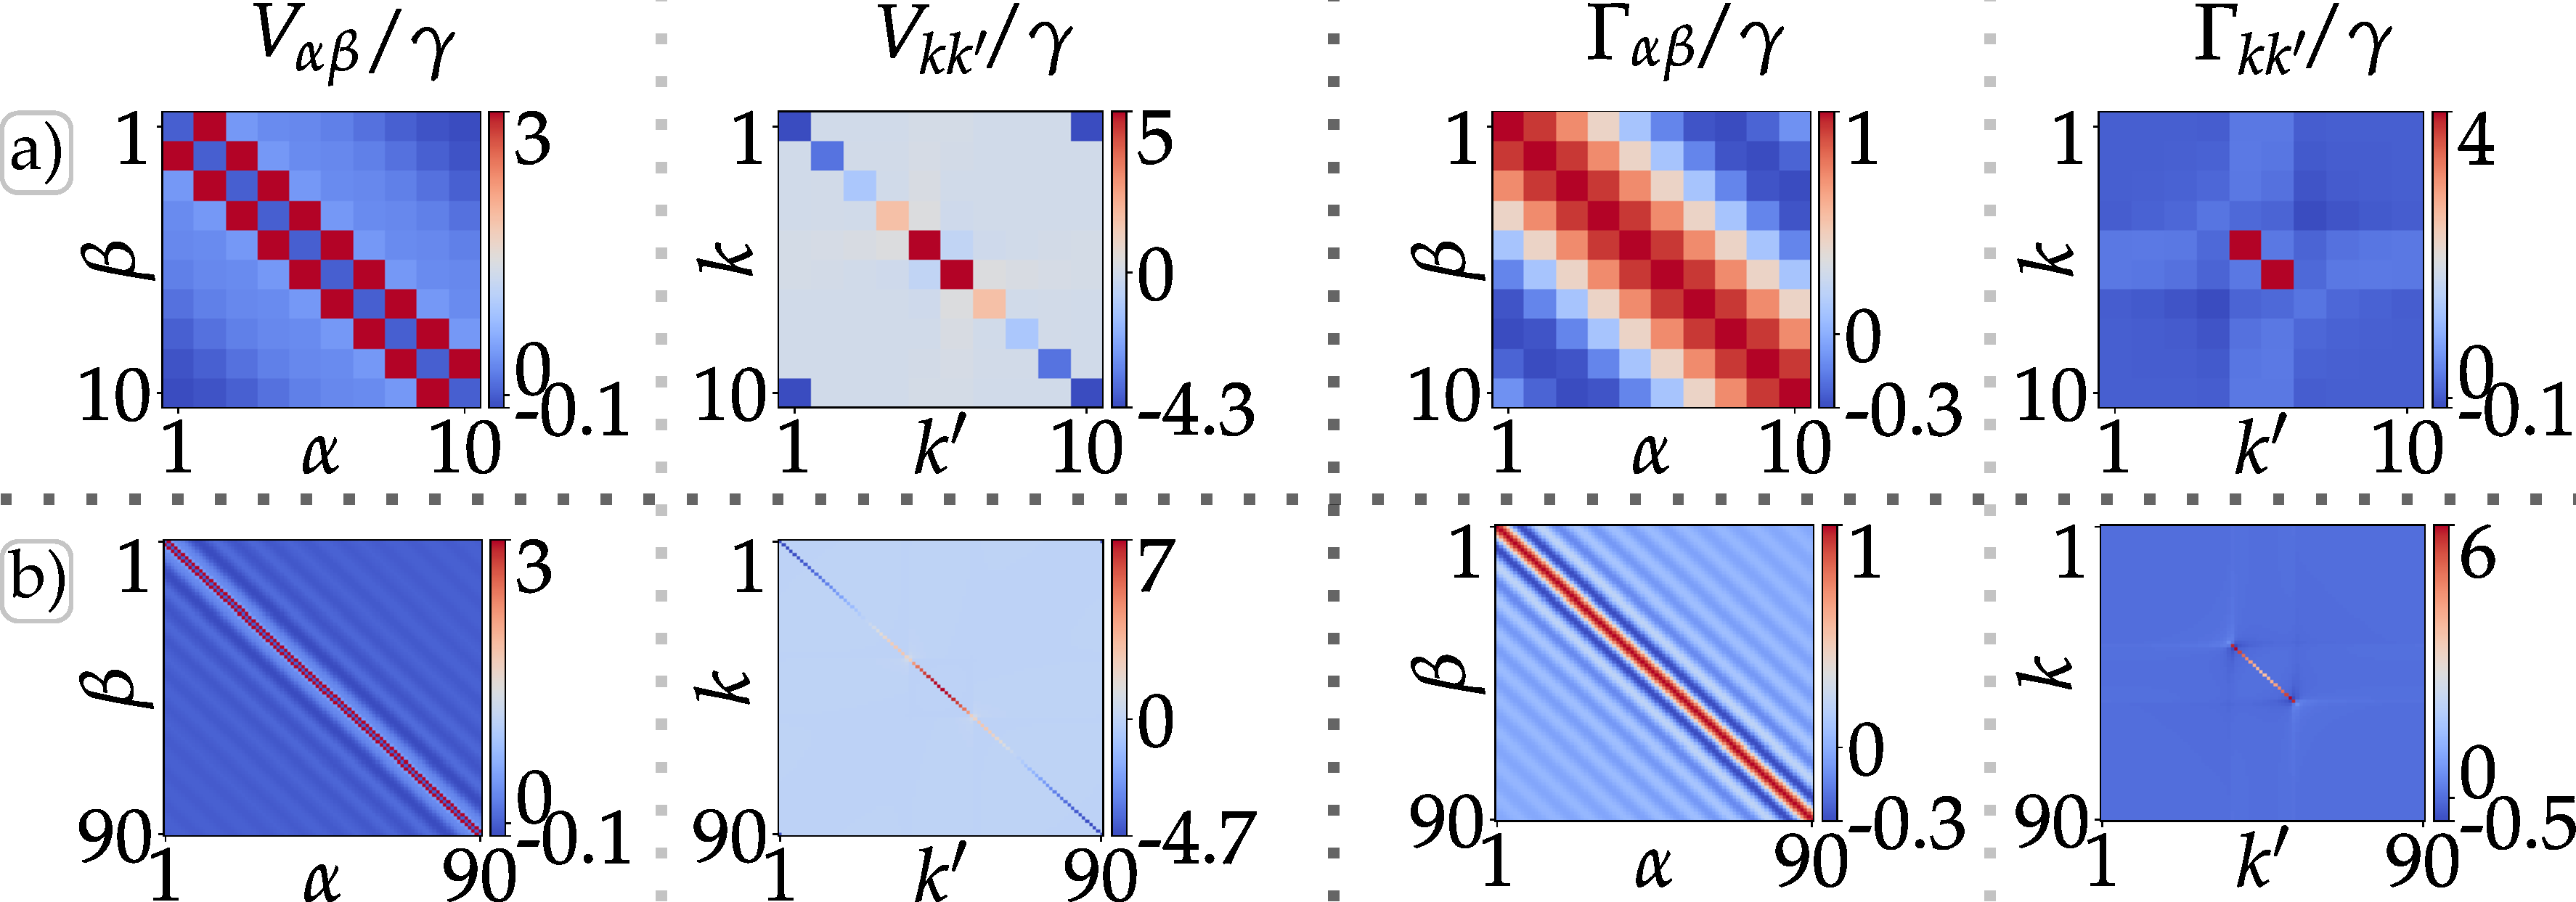
\includegraphics[width=1.0\textwidth]{V_matrix_Real_and_k_space}
    \caption{\textbf{a)} Chain of $N = 10 $ atoms.
    \textbf{b)} Chain of $N = 90 $ atoms.
    The atomic dipoles are aligned and perpendicular to the chain, and the interatomic distance is chosen to be $ d = 0.1 \lambda $.
    The interaction matrix $ (V)_{\alpha \beta} $ and $ (\Gamma)_{\alpha \beta} $ are displayed in units of $ \gamma $.
    Left side in real space and right side in $k$-space.}
    \label{fig:Diagonalizable}
\end{figure}